
\chapter{Supplementary Material}

%\begin{figure}
%\includegraphics[width=1\textwidth]{RhoShortPic.png}
%\end{figure}

 \begin{figure}[h!]
\centering
  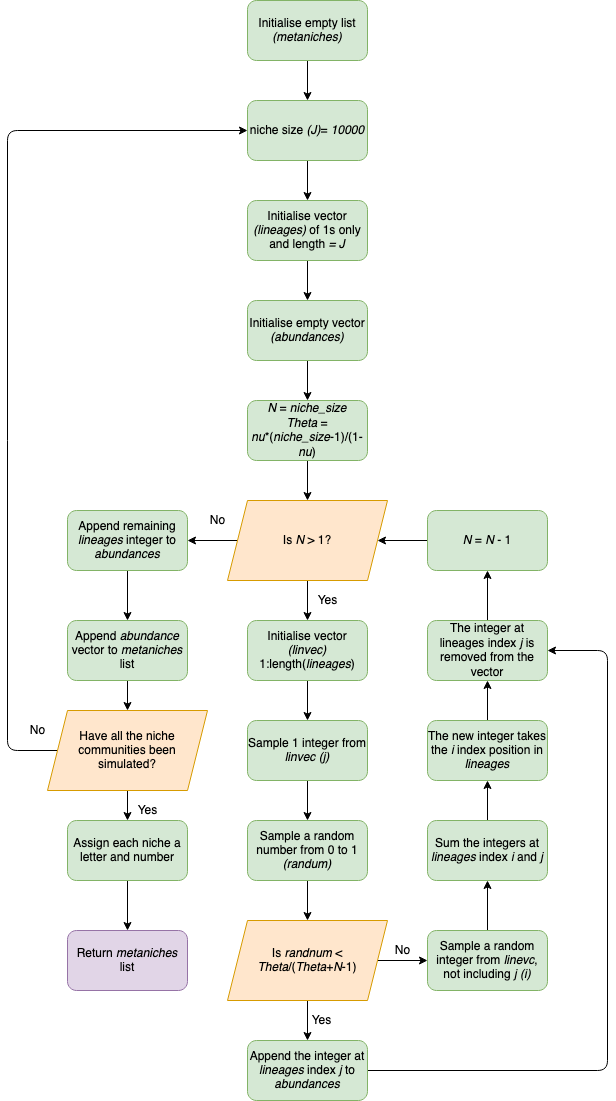
\includegraphics[scale=0.4]{metacommunity.png}
  \caption{Flowchart of metacommunity function}
  \label{fig:Flowchart}
\end{figure}

\begin{table}[h]
    \caption{Summary of Datasets}
    \label{crouch}
    \begin{tabular}{  l  p{5cm} p{1.5cm}  p{3cm} p{3cm}}
        \toprule
\textbf{Study and Dataset ID} 
&\textbf{Author and Year}      
& \textbf{Habitat}
& \textbf{Taxa}   \\\midrule
Study 1, Datasets 1 \& 2
&\cite{li2020island}
& Terrestrial
& Bacteria \& Fungi \\\hline
Study 2, Dataset 3
&\cite{battes2019species} 
& Lacustrine
&Algae \\\hline
Study 3, Datasets 4-15
&\cite{darcy2018island} 
& Lacustrine
&Bac, Alg, Fungi \& Proto \\\hline
Study 4, Datasets 16 \& 17
&\cite{delgado2018experimentally} 
& Terrestrial
& Bacteria \\\hline
Study 5, Dataset 18
&\cite{davison2018microbial} 
& Terrestrial
& Fungi \\\hline
Study 6, Datasets 19 \& 20
&\cite{glassman2017theory} 
& Plant
& Fungi \\\hline
Study 7, Dataset 21
&\cite{varbiro2017functional} 
& Lacustrine
& Algae \\\hline
Study 8, Datasets 22 \& 23
&\cite{kavazos2016small} 
& Lacustrine
& Bac \& Proto \\\hline
Study 9, Dataset 24
&\cite{bolgovics2016species} 
& Lacustrine
& Algae \\\hline
Study 10, Datasets 25-27
&\cite{article} 
& Lacustrine
& Alg, Proto \& Fun \\\hline
Study 11, Datasets 28-32
&\cite{jean2016equilibrium} 
& Terrestrial
& Bac, Path, Fun \& Proto \\\hline
Study 12, Dataset 33
&\cite{cashdan2014biogeography} 
& Terrestrial
& Pathogens \\\hline
Study 13, Dataset 34
& \cite{LepereCecile2013Gdae}
& Lacustrine
&Protozoa \\\hline
Study 14, Datasets 35 \& 36
& \cite{LanzenAnders2013SPaE}
& Lacustrine
& Bacteria \& Archaea \\\hline
Study 15, Dataset 37
&\cite{RENGEFORSK2012Plma} 
& Lacustrine
& Algae \\\hline
Study 16, Datasets 38-39
&\cite{FeinsteinLarryM2012Tran} 
& Plant
& Fungi \\\hline
Study 17, Dataset 40
&\cite{StompMaayke2011Lbpi} 
& Lacustrine
& Algae \\\hline
Study 18, Dataset 41
&\cite{JohnL.Orrock2011BaER} 
& Terrestrial
& Pathogens \\\hline
Study 19, Datasets 42 \& 43
&\cite{barberan2011euxinic} 
& Lacustrine
& Bacteria \\\hline
Study 20, Dataset 44
&\cite{peay2007strong} 
& Plant
& Fungi \\\hline
Study 21, Dataset 45
&\cite{van2006bacterial} 
& Machine
& Bacteria \\\hline
Study 22, Dataset 46
&\cite{bell2005larger} 
& Lacustrine
& Bacteria \\\hline
Study 23, Dataset 47
&\cite{reche2005does} 
& Lacustrine
& Bacteria \\\hline
Study 24, Datasets 48-50
&\cite{van2005island} 
& Machine
& Bacteria \\\hline
Study 25, Dataset 51
&\cite{karatayev2005community} 
& Lacustrine
& Algae \\\hline
Study 26, Datasets 52 \& 53
&\cite{mccormick1988comparison} 
& Riverine
& Protozoa and Algae \\\hline
Study 27, Dataset 54
&\cite{wildman1987fungal} 
& Terrestrial
& Fungi \\\hline
Study 28, Dataset 55
&\cite{henebry1980effect} 
& Lacustrine
& Protozoa \\\hline
Study 29, Datasets 56 \& 57
&\cite{patrick1967effect} 
& Riverine
& Algae \\
        \bottomrule
    \end{tabular}
\end{table}

\begin{table}[h]
    \caption{Rho Estimation Methods (S \& D ID = Study \& Dataset ID)}
    \label{crouch}
    \begin{tabular}{  l  p{2cm} p{2cm}  p{1.5cm} p{5cm} p{5cm}}
        \toprule
\textbf{Study/Data}   
&\textbf{Taxa}
&\textbf{Habitat}   
& \textbf{$\rho$ (cm\textsuperscript{3})}   
& \textbf{Method} \\\midrule
S1, D1 
& Bacteria
& Soil
& 1.48x10\textsuperscript{12}   
& Gene seq num from paper \\\hline
S1, D2   
& Fungi
& Soil
& 7.41x10\textsuperscript{3}              
& Gene seq num from paper \\\hline
S2, D3  
&Algae
&Freshwater
& 3.56x10\textsuperscript{3}   
& Proxy \cite{pasztaleniec2010phytoplankton} \\\hline
S3, D4-6  
&Bacteria
&Cryo Holes
& 4.50x10\textsuperscript{4}   
& Proxy \cite{cameron2012structure} \\\hline
S3, D7-9  
&Algae
&Cryo Holes
& 1 
& Gene seq num from paper \\\hline
S3, D10-12  
&Fungi
&Cryo Holes
& 1  
& Gene seq num from paper \\\hline
S3, D13-15  
&Protozoa
&Cryo Holes
& 1   
& Gene seq num from paper \\\hline
S4, D16 
&Bacteria
&Soil
& 3.50x10\textsuperscript{12} 
& Gene seq num from paper \\\hline
S4, D17 
&Bacteria
&Soil
& 1.48x10\textsuperscript{13}  
& Gene seq num from paper \\\hline
S5, D18 
&Fungi
&Soil
& 1     
& 1 as area includes entire island \\\hline
S6, D19 \& 20 
&Fungi
&Soil
& 2.98x10\textsuperscript{3}   
& Gene seq num from paper \\\hline
S7, D21 
&Algae
&Freshwater 
& 3.56x10\textsuperscript{3}   
& Same proxy as D3 \\\hline
S8, D22
&Bacteria
&Sal Water
& 3.00x10\textsuperscript{6}    
& Proxy \cite{anton2000extremely} \\\hline
S8, D23 
&Protozoa
&Sal Water
& 1.84x10\textsuperscript{2}          
& Proxy \cite{elloumi2006composition} \\\hline
S9, D24 
&Algae
&Freshwater 
& 3.56x10\textsuperscript{3}               
& Same proxy as D3 \\\hline
S10, D25 
&Algae 
&Freshwater
& 3.56x10\textsuperscript{3}             
& Same proxy as D3 \\\hline
S10, D26 
&Protozoa
&Freshwater 
& 1.92x10\textsuperscript{3}      
& Proxy \cite{olive2020control} \\\hline
S10, D27
&Fungi
&Freshwater
& 1         
& Proxy \cite{wurzbacher2010fungi} \\\hline
S11, D28-32
&Bac, Pat, Fun, Pro
&Hosts
& 1            
& 1 as area includes entire island \\\hline
S12, D33
&Pathogens
&Hosts
& 1        
& 1 as area includes entire island \\\hline
S13, D34
&Protozoa
&Freshwater 
& 5.72x10\textsuperscript{3} 
& Nanoflag count taken from paper \\\hline
S14, D35
&Archaea
&Sal Water
& 1.00x10\textsuperscript{7} 
& Book \cite{kulkarni2019alkaliphiles} \\\hline
S14, D36
&Bacteria
&Sal Water 
& 6.00x10\textsuperscript{6} 
& Proxy \cite{humayoun2003depth} \\\hline
S15, D37
&Algae
&Sal Water
& 4.85x10\textsuperscript{3} 
& Proxy \cite{rengefors2008marine} \\\hline
S16, D38-39
&Fungi
&Plant
& 10       
& No proxy found so 10 est \\\hline
S17, D40
&Algae
&Freshwater
& 3.56x10\textsuperscript{3}   
& Same proxy as D3 \\\hline
S18, D41
&Pathogens
&Hosts
& 1     
& 1 as area includes entire island \\\hline
S19, D42 \& 43
&Bacteria
&Freshwater
& 1.16x10\textsuperscript{7} 
& Proxy \cite{cole1993bacterial} \\\hline
S20, D44
&Fungi
&Soil
& 6.90x10\textsuperscript{6} 
& Proxy \cite{prevost2011validation} \\\hline
S21, D45
&Bacteria
&Machine
& 2.29x10\textsuperscript{10} 
& Cell abund taken from paper \\\hline
S22, D46
&Bacteria
&Tree Holes
& 4.90x10\textsuperscript{5} 
& Proxy \cite{rivett2018abundance} \\\hline
S23, D47
&Bacteria
&Freshwater
& 1.16x10\textsuperscript{7} 
& Same proxy as D43 \\\hline
S24, D48-50
&Bacteria
&Machine
& 2.29x10\textsuperscript{10}  
& Same proxy as D46 \\\hline
S25, D51
&Algae
&Freshwater
& 3.56x10\textsuperscript{3}    
& Same proxy as D3 \\\hline
S26, D52
&Protozoa
&River
& 5.72x10\textsuperscript{3} 
& Same proxy as D34 \\\hline
S26, D53
&Algae
&River
& 3.56x10\textsuperscript{3}    
& Same proxy as D3 \\\hline
S27, D54
&Fungi
&Soil
& 1.00x10\textsuperscript{5} 
& Book \cite{pepper2019biotic} \\\hline
S28, D55
&Protozoa
&Freshwater
& 5.72x10\textsuperscript{3} 
& Same proxy as D34 \\\hline
S29, D56 \& 57
&Algae
&River 
& 3.56x10\textsuperscript{3}   
& Same proxy as D3 \\
        \bottomrule
    \end{tabular}
\end{table}

\begin{figure}[htbp]
\centering
\subfloat[Dataset 4, bacteria in Antarctic Croconite Holes]{\label{fig:a}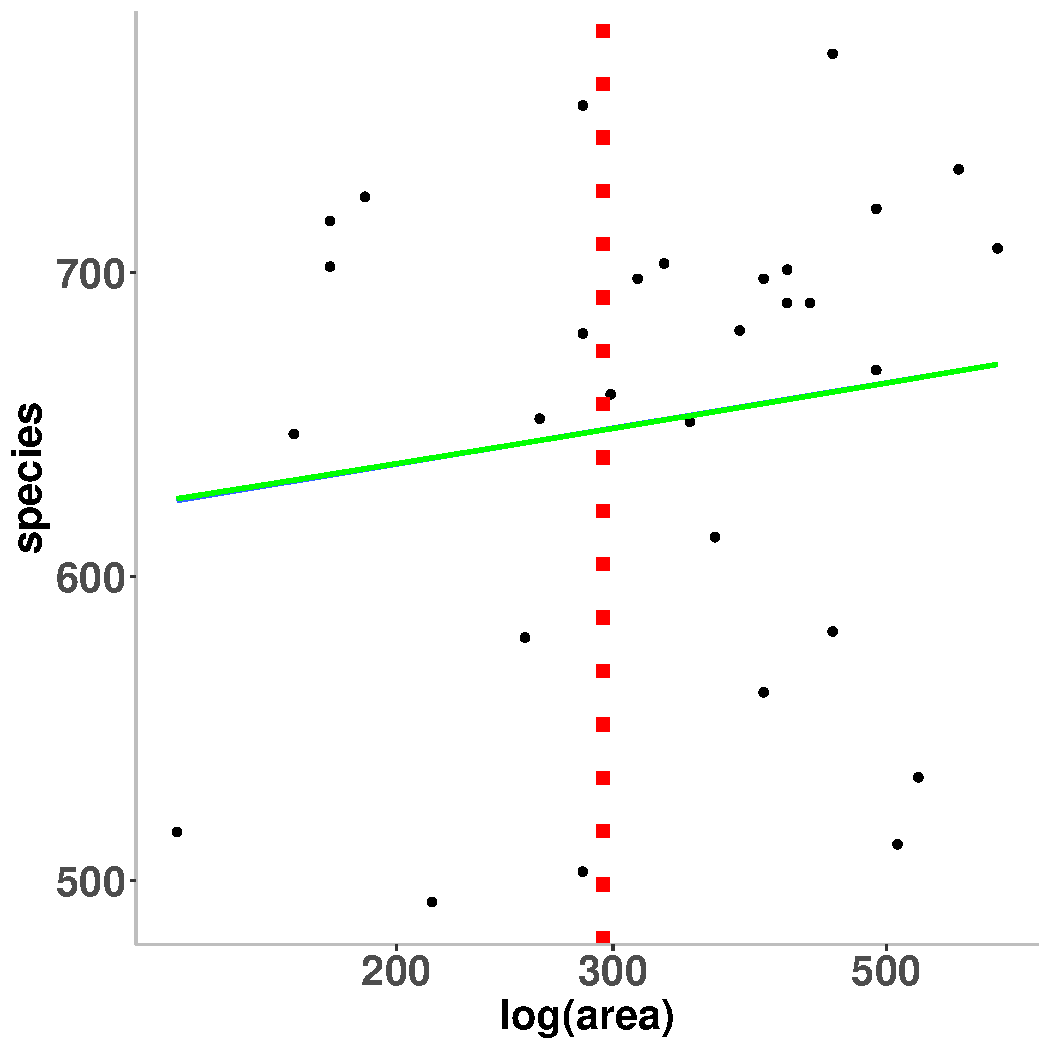
\includegraphics[width=0.45\linewidth]{../Results/ClassicNLLSPlot4.pdf}}\qquad
\subfloat[Dataset 54, fungi in a soil based laboratory experiment]{\label{fig:b}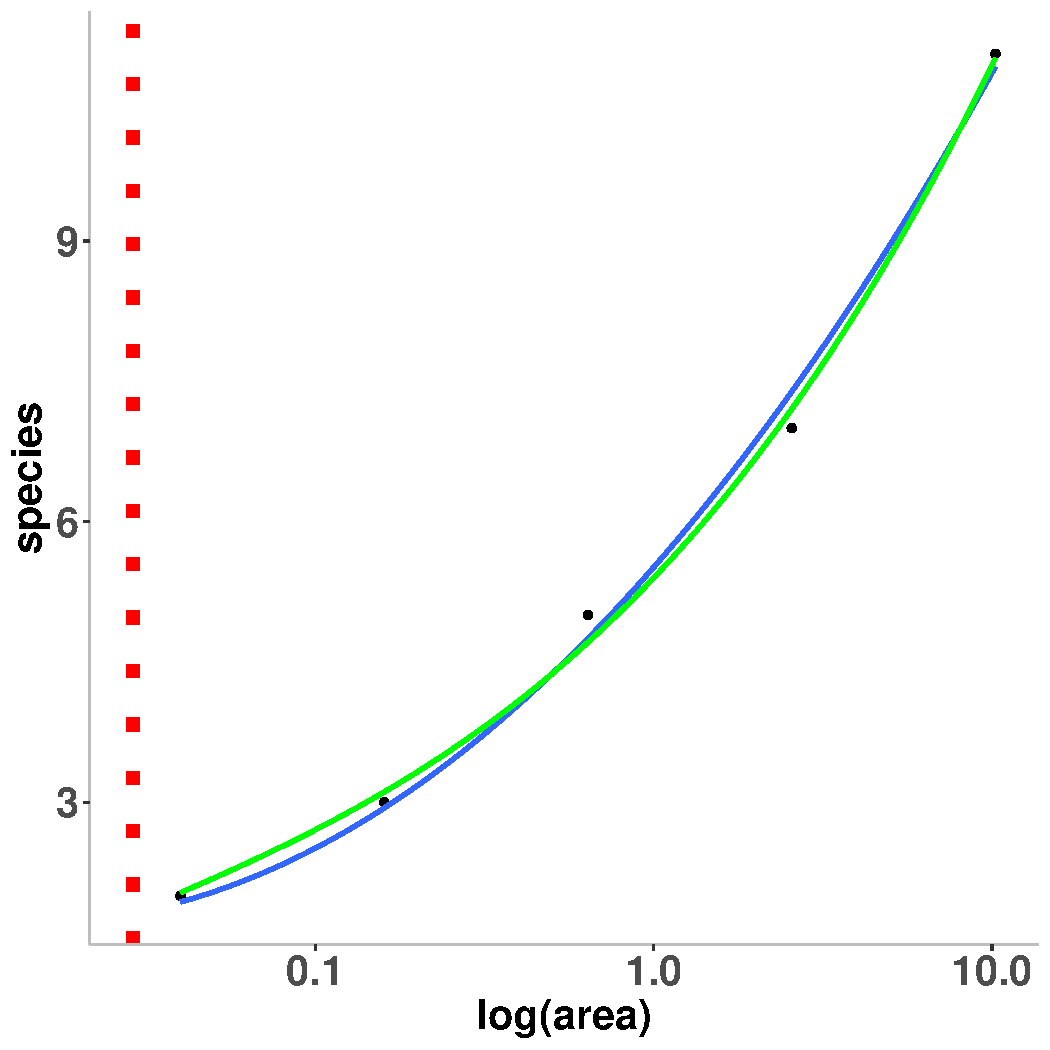
\includegraphics[width=0.45\linewidth]{../Results/PeriNLLSPlot48.pdf}}\\
\subfloat[Dataset 22, benthic bacteria in saline lakes (log area plotted with depth)]{\label{fig:c}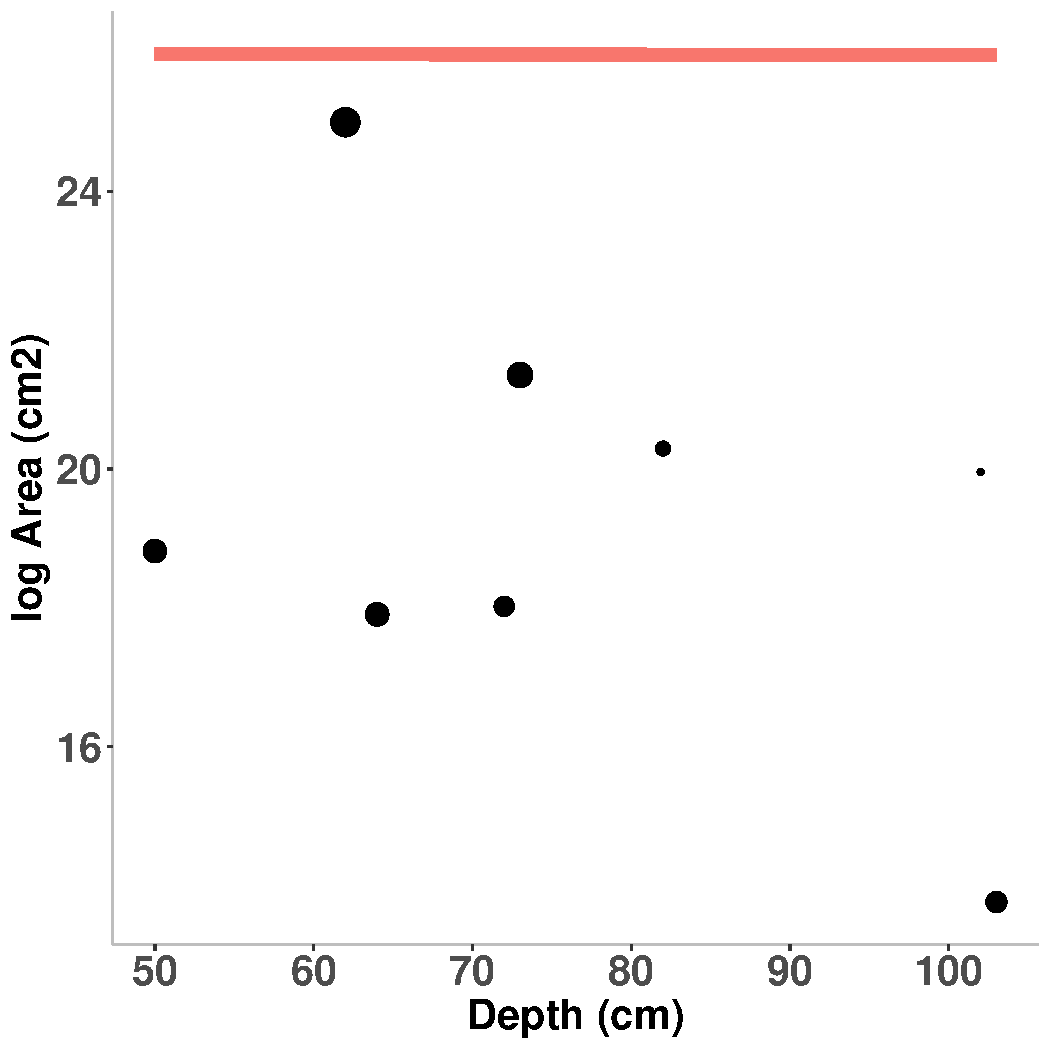
\includegraphics[width=0.45\textwidth]{../Results/DepthNLLSPlot19.pdf}}\qquad%
\subfloat[Dataset 22, benthic bacteria in saline lakes (log volume plotted with OTU richness)]{\label{fig:d}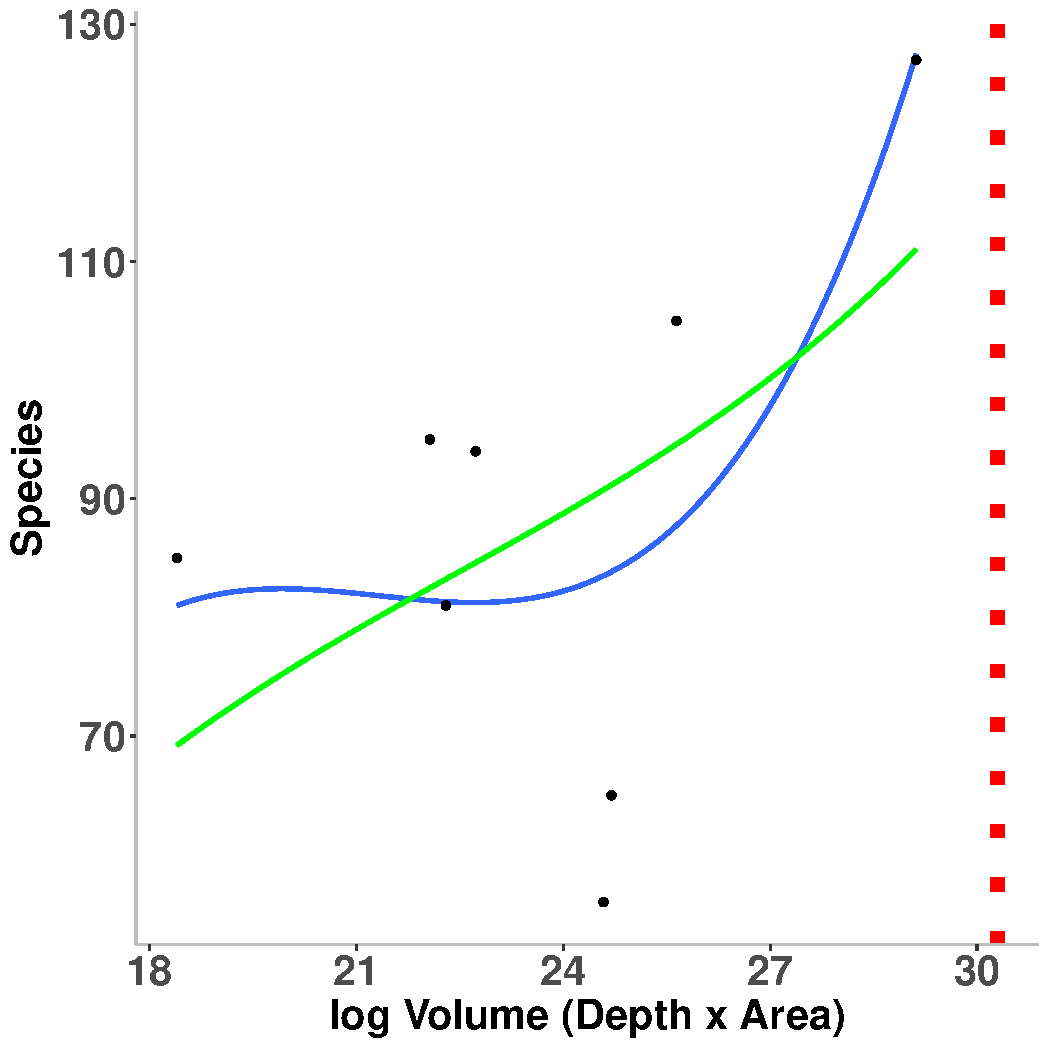
\includegraphics[width=0.45\textwidth]{../Results/DepthNLLSPlot2_19.pdf}}%
\bigskip

Simulation data point \tikz\draw[black,fill=black] (0,0) circle (.5ex); \;\;NLLS fit \textcolor{blue}{\rule{1.5cm}{1mm}} \;\;Power-Law fit \textcolor{green}{\rule{1.5cm}{1mm}}\;\; \textit{A\textsubscript{crit}/A\textsubscript{vol}}\;\; \textcolor{red}{\rule{0.1cm}{1mm}}\; \textcolor{red}{\rule{0.1cm}{1mm}}\; \textcolor{red}{\rule{0.1cm}{1mm}}\; \textcolor{red}{\rule{0.1cm}{1mm}}\\

\caption{Selection of plots of datasets that failed to be fit using either of the three model variants (Classic, Depth, Perimeter) or the power-law model, where the blue line is the model fit, the green line is the power-law model fit and the red dotted line is the \textit{A\textsubscript{crit}} estimation. A) Dataset 4, bacteria in cryoconite holes with the Classic Model (NLLS fit: R\textsubscript{2}=0.02, adjusted R\textsubscript{2}=-0.13, $\theta$=29, \textit{m\textsubscript{0}}=0.208, \textit{K}=354, \textit{A\textsubscript{crit}}=294 cm\textsuperscript{2}, power-law fit: R\textsubscript{2}=0.02, adjusted R\textsubscript{2}=-0.14, \textit{z}=0.04, \textit{c}=5.03). B) Fungi in soil based laboratory experiment plotted with the Perimeter Model (R\textsubscript{2}=0.099, adjusted R\textsubscript{2}=Inf, $\theta$=6, \textit{m\textsubscript{0}}=6.24 x 10\textsuperscript{-6}, \textit{K}=1, \textit{A\textsubscript{crit}}=2.89 x 10\textsuperscript{-2} cm\textsuperscript{2}, power-law fit: R\textsubscript{2}=0.99, adjusted R\textsubscript{2}=-Inf, \textit{z}=0.30, \textit{c}=5.41). C) Benthic bacteria in saline lakes plotted with the Depth Model (R\textsubscript{2}=0.51, adjusted R\textsubscript{2}=-0.15, $\theta$=14, \textit{m\textsubscript{0}}=1.98 x 10\textsuperscript{-16}, \textit{K}=81, \textit{A\textsubscript{crit}}=1.89 x 10\textsuperscript{11} cm\textsuperscript{2}, power-law fit: R\textsubscript{2}=0.24, adjusted R\textsubscript{2}=-0.77, \textit{z}=0.04, \textit{c}=39)}
\label{fig:myfig}
\end{figure}


\begin{table}[h]
    \caption{Results of successful Power-Law Model fitting to the 24 positive TAR datasets with R\textsuperscript{2}, adjusted R\textsuperscript{2}, \textit{z} values (model exponent), \textit{c} values (model constant) (S \& D ID = Study \& Dataset ID)}
    \label{crouch}
    \begin{tabular}{  l  p{6cm} p{1cm}  p{1cm} p{1cm} p{1cm}}
        \toprule
\textbf{S \& D ID} 
&\textbf{Author \& Year}
&\textbf{R\textsuperscript{2}}      
& \textbf{Adj R\textsuperscript{2}}
& \textit{z}  
& \textit{c}\\\midrule
S1, D1
&\cite{li2020island}
& 0.56
& 0.49
& 0.09
& 1294.63 \\\hline
S1, D2
&\cite{li2020island}
& 0.60
& 0.53
& 0.10
& 332.03 \\\hline
S3, D6
&\cite{darcy2018island} 
& 0.23
& 0.10
& 0.32
& 70.02 \\\hline
S3, D11
&\cite{darcy2018island} 
& 0.27
& 0.15
& 0.42
& 4.68\\\hline
S4, D16
&\cite{delgado2018experimentally} 
& 0.82
& 0.75
& 0.11
& 340.96 \\\hline
S4, D17
&\cite{delgado2018experimentally} 
& 0.70
& 0.54
& 0.08
& 451.61 \\\hline
S6, D19
&\cite{glassman2017theory} 
& 0.23
& 0.02
& 0.27
& 0.48 \\\hline
S6, D20
&\cite{glassman2017theory} 
& 0.32
& 0.13
& 0.16
& 1.93 \\\hline
S7, D21
&\cite{varbiro2017functional} 
& 0.02
& 0.0001
& 0.01
& 23.10 \\\hline
S9, D24
&\cite{bolgovics2016species} 
& 0.62
& 0.48
& 0.05
& 32.25 \\\hline
S10, D25
&\cite{article} 
& 0.38
& 0.28
& 0.06
& 48.28 \\\hline
S10, D26 
&\cite{article} 
& 0.29
& 0.17
& 0.14
& 0.29 \\\hline
S11, D28
&\cite{jean2016equilibrium} 
& 0.23
& 0.18
& 0.01
& 39.29 \\\hline
S11, D29
&\cite{jean2016equilibrium} 
& 0.34
& 0.30
& 0.02
& 19.31 \\\hline
S11, D30
&\cite{jean2016equilibrium} 
& 0.24
& 0.19
& 0.02
& 4.27 \\\hline
S11, D31 
&\cite{jean2016equilibrium} 
& 0.35
& 0.31
& 0.03
& 4.60 \\\hline
S11, D32
&\cite{jean2016equilibrium} 
& 0.33
& 0.29
& 0.05
& 4.26 \\\hline
S20, D44
&\cite{peay2007strong} 
& 0.87
& 0.78
& 0.18
& 0.64 \\\hline
S21, D45
&\cite{van2006bacterial} 
& 0.94
& 0.82
& 0.27
& 0.88 \\\hline
S22, D46
&\cite{bell2005larger} 
& 0.46
& 0.38
& 0.33
& 1.74 \\\hline
S24, D48
&\cite{van2005island} 
& 0.73
& 0.63
& 0.36
& 1.25 \\\hline
S24, D49
&\cite{van2005island} 
& 0.84
& 0.76
& 0.32
& 1.80 \\\hline
S24, D50
&\cite{van2005island} 
& 0.80
& 0.73
& 0.36
& 1.34 \\\hline
S25, D51
&\cite{karatayev2005community} 
& 0.10
& 0.09
& 0.11
& 19.00  \\
        \bottomrule
    \end{tabular}
\end{table}

\begin{table}[h]
    \caption{Results of Power-Law Model AIC score - Classic, Depth and Perimeter AIC scores. There must be a difference of at least 2 to be statistically significant (positive results favour the Classic, Depth and Perimeter Models, negative results favour the Power-Law Model) (S \& D ID = Study \& Dataset ID)}
    \label{crouch}
    \begin{tabular}{  l  p{6cm} p{1cm}  p{1cm} p{1cm} p{1cm}}
        \toprule
\textbf{S \& D ID} 
&\textbf{Author \& Year}
&\textbf{Classic}      
& \textbf{Depth}
& \textbf{Perimeter} \\\midrule
S1, D1
&\cite{li2020island}
& 7.25
& 7.25
& 6.91 \\\hline
S1, D2
&\cite{li2020island}
& 10.37
& 10.18
& 9.49 \\\hline
S3, D6
&\cite{darcy2018island} 
& 0.23
& 0.23
& 0.08 \\\hline
S3, D11
&\cite{darcy2018island} 
& 0.005
& 0.02
& 0.02\\\hline
S4, D16
&\cite{delgado2018experimentally} 
& 0.005
& 0.005
& 0.005 \\\hline
S4, D17
&\cite{delgado2018experimentally} 
& 0.002
& 0.002
& 0.002 \\\hline
S6, D19
&\cite{glassman2017theory} 
& 0.03
& 0.03
& 0.01 \\\hline
S6, D20
&\cite{glassman2017theory} 
& 0.72
& 0.72
& 0.52 \\\hline
S7, D21
&\cite{varbiro2017functional} 
& 1.20
& 1.22
& 1.03 \\\hline
S9, D24
&\cite{bolgovics2016species} 
& 2.64
& 2.62
& 3.33 \\\hline
S10, D25
&\cite{article} 
& 0.91
& 1.03
& 0.92 \\\hline
S10, D26 
&\cite{article} 
& 0.05
& 0.11
& 0.04 \\\hline
S11, D28
&\cite{jean2016equilibrium} 
& 0.49
& 0.49
& -0.61 \\\hline
S11, D29
&\cite{jean2016equilibrium} 
& 0.33
& 0.34
& 0.11 \\\hline
S11, D30
&\cite{jean2016equilibrium} 
& 2.77
& 2.78
& 3.16 \\\hline
S11, D31 
&\cite{jean2016equilibrium} 
& 0.76
& 0.75
& -0.05 \\\hline
S11, D32
&\cite{jean2016equilibrium} 
& 2.22
& 2.21
& 0.75 \\\hline
S20, D44
&\cite{peay2007strong} 
& -0.05
& -0.05
& -0.27 \\\hline
S21, D45
&\cite{van2006bacterial} 
& 2.67
& 2.67
& 2.25 \\\hline
S22, D46
&\cite{bell2005larger} 
& 0.45
& 1.34
& 0.17 \\\hline
S24, D48
&\cite{van2005island} 
& 2.84
& 2.87
& 0.47 \\\hline
S24, D49
&\cite{van2005island} 
& 4.28
& 4.33
& 1.80 \\\hline
S24, D50
&\cite{van2005island} 
& 3.38
& 3.42
& 0.59 \\\hline
S25, D51
&\cite{karatayev2005community} 
& 0.23
& -1.18
& 0.17  \\
        \bottomrule
    \end{tabular}
\end{table}

\begin{table}[h]
    \caption{Best-fit results of the Classic, Depth and Perimeter Model fittings, with best-fit parameters ($\theta$, \textit{m\textsubscript{0}}, \textit{K}), \textit{A\textsubscript{crit}} and best-fit model (S \& D ID = Study \& Dataset ID)}
    \label{crouch}
    \begin{tabular}{  l  p{1cm}  p{1cm} p{1.5cm} p{1.5cm} p{1.5cm} p{1.5cm} p{1.5cm}}
        \toprule
\textbf{S \& D ID} 
&R\textsuperscript{2}
& Adj R\textsuperscript{2}
& $\theta$
& \textit{m\textsubscript{0}}
& \textit{K}
& \textit{A\textsubscript{crit}}
& Best-fit Model\\\midrule
S1, D1
& 0.65
& 0.60
& 1.73x10\textsuperscript{3}
& 3.67x10\textsuperscript{-5}
& 1
& 5.00x10\textsuperscript{-2}
& All \\\hline
S1, D2
& 0.72
& 0.67
& 3.56x10\textsuperscript{2}
& 1.80x10\textsuperscript{-8}
& 1
& 4.21x10\textsuperscript{2}
&Classic \& Depth \\\hline
S3, D6
& 0.23
& 0.11
& 1.60x10\textsuperscript{5}
& 2.43x10\textsuperscript{-5}
& 204
& 1.98x10\textsuperscript{2}
& All \\\hline
S3, D11
& 0.27
& 0.15
& 5.89x10\textsuperscript{4}
& 5.64x10\textsuperscript{-1}
& 25
& 1.92x10\textsuperscript{2}
& All \\\hline
S4, D16
& 0.82
& 0.75
& 1.42x10\textsuperscript{2}
& 1.53x10\textsuperscript{-12}
& 315
& 5.52x10
&  All \\\hline
S4, D17
& 0.70
& 0.54
& 1.08x10\textsuperscript{2}
& 5.12x10\textsuperscript{-13}
& 424
& 5.02x10\textsuperscript{2}
&  All \\\hline
S6, D19 
& 0.23
& 0.02
& 13
& 5.88x10\textsuperscript{-7}
& 4
& 1.91x10\textsuperscript{4}
& All \\\hline
S6, D20
& 0.34
& 0.17
& 2
& 5.09x10\textsuperscript{-8}
& 1
& 4.91x10\textsuperscript{2}
&  Classic \& Depth \\\hline
S7, D21
& 0.02
& 0.01
& 1
& 1.39x10\textsuperscript{-4}
& 21
& 1.03x10\textsuperscript{20}
& Classic \& Depth \\\hline
S9, D24
& 0.69
& 0.58
& 16
& 2.79x10\textsuperscript{-8}
& 60
& 4.83x10\textsuperscript{10}
& Perimeter \\\hline
S10, D25
& 0.41
& 0.31
& 10
& 1.19x10\textsuperscript{-6}
& 2
& 2.38x10
& Depth \\\hline
S10, D26  
& 0.29
& 0.18
& 1
& 2.86x10\textsuperscript{-13}
& 3
& 1.33x10\textsuperscript{9}
& Classic \& Depth \\\hline
S11, D28
& 0.23
& 0.18
& 1
& 1.70x10\textsuperscript{-12}
& 51
& 1.07x10\textsuperscript{48}
&  Classic \& Depth \\\hline
S11, D29
& 0.34
& 0.30
& 1
& 3.75x10\textsuperscript{-6}
&28
& 1.89x10\textsuperscript{31}
&  All \\\hline
S11, D30
& 0.28
& 0.23
& 2.43x10\textsuperscript{3}
& 5.87x10\textsuperscript{-10}
& 7
& 8.52x10\textsuperscript{16}
&  Perimeter \\\hline
S11, D31 
& 0.36
& 0.32
& 1
& 3.31x10\textsuperscript{-13}
& 9
& 2.23x10\textsuperscript{24}
& Classic \\\hline
S11, D32
& 0.35
& 0.31
& 3
& 1.44x10\textsuperscript{-15}
& 17
& 4.24x10\textsuperscript{16}
&  Classic \& Depth \\\hline
S20, D44
& 0.85
& 0.77
& 5
& 6.15x10\textsuperscript{-11}
& 2
& 4.08x10\textsuperscript{4}
&  All \\\hline
S21, D45
& 0.96
& 0.88
& 9
& 4.97x10\textsuperscript{-16}
& 7
& 2.62x10\textsuperscript{4}
& Classic \& Depth \\\hline
S22, D46
& 0.49
& 0.40
& 8
& 3.75x10\textsuperscript{-9}
& 6
& 2.19x10\textsuperscript{2}
& Depth \\\hline
S24, D48
& 0.78
& 0.69
& 7
& 7.97x10\textsuperscript{-14}
& 1
& 1.95x10
& Classic \& Depth \\\hline
S24, D49
& 0.89
& 0.83
& 6
& 1.15x10\textsuperscript{-13}
& 1
& 1.38x10
&  Classic \& Depth\\\hline
S24, D50
& 0.84
& 0.78
& 7
& 8.74x10\textsuperscript{-14}
& 1
& 1.78x10
& Classic \& Depth\\\hline
S25, D51
& 0.10
& 0.09
& 12
& 3.25x10\textsuperscript{-5}
& 28
& 4.46x10\textsuperscript{3}
& All \\
        \bottomrule
    \end{tabular}
\end{table}


